\section{Численные методы решения}
\label{sec:algrhtms}

Далее мы опишем алгоритмы использующиеся для решений уравнений
эйконала. Это два разных метода, базирующиеся на разных и идеях и,
следовательно, пригодные для разных целей. Один заточен для
максимального ускорения работы и, как это часто бывает с такими
алгоритмами практически неспособен к параллелизации, другой же --
наоборот работает несколько медленнее, но гораздо проще поддается
распараллеливанию.

\subsection{Общая идея методов}
\label{sec:general-idea}

Для всех методов нам необходимо научится решать задачу в локальном
случае. Разберем для начала одномерный случай. Пусть нам дано
следующее уравнение эйконала:

\begin{equation}
  \label{eq:eik_smp}
  \sqrt{(\frac{dT}{dx})^2}=F(x), T(-1) = T(1) = 0.
\end{equation}


% Вставить куда-нибудь ссылку
Для упрощения обозначений мы запишем производную $T$ по $x$ в виде
$T_x$. Также в будущем мы будем поступать и для частных
производных. После преобразования уравнение~\eqref{eq:eik_smp} примет вид:

\begin{equation*}
  \sqrt{T_x^2}=F(x), T(-1) = T(1) = 0.
\end{equation*}


Имеется функция скорости $F(x) > 0$, требуется построить
решение $T(x)$. Мы видим, что решение не уникально (если t(x) решает
задачу, то тогда и $-t(x)$ также ее решает). Будем работать только с
положительными решениями.

Рассмотрим обыкновенное дифференциальное уравнение и разобьем решение
на подзадачи:

\begin{equation*}
  \begin{cases}
      \begin{array}{ll}
        T_x = ~F(x), \quad x \ge 0,\\
        T_x = -F(x), \quad x \le 0,\\[0.3cm]
        T(-1)= T(1) = 0.
      \end{array}
    \end{cases}
\end{equation*}

Для численной аппроксимации разобьем ось $x$ на набор точек сетки
$x_i=i\Delta x$. Положим $T_i = T(i \Delta x)$ и $F_i = F(i \Delta
x)$, где $\Delta x$ - это шаг дискретизации, $i = -n, \cdots,
n$. 

введем также обозначение для разностных производных первого порядка 1-го порядка:

\begin{eqnarray*}
    D^{+x}_iT(x_i) &=& \frac{T_{i+1} - T_{i}}{\Delta x} \\
    D^{-x}_iT(x_i) &=& \frac{T_{i} - T_{i-1}}{\Delta x}
\end{eqnarray*}

Далее используем разложение Тейлора и отбросим остаток. Получим
следующую дискретную систему:


\begin{equation}
  \label{eq:discretise}
  \begin{cases}
      T_n = 0,\\
      D^{+x}_iT(x_i) = F_i, \quad i>0 \\
      D^{-x}_iT(x_i)  = F_i, \quad i>0\\
      T(-n) = 0\\
    \end{cases}
\end{equation}

Отметим, что
\begin{itemize}
\item[ ] $T_{n-1}$ может быть получено из $T_n$
\item[ ] $T_{n-2}$ может быть получено из $T_{n-1}$
\item[ ]  $\cdots$
\item[ ] $T_{1}$ может быть получено из $T_2$
\item[ ] $T_{0}$ может быть получено из $T_{1}$
\item[ ]  $\cdots$
\item[ ] $T_{-n+1}$ может быть получено из $T_{-n}$
\item[ ] $T_{-n+2}$ может быть получено из $T_{-n+1}$
\item[ ]  $\cdots$
\item[ ] $T_{-1}$ может быть получено из $T_{-2}$
\item[ ] $T_{0}$ может быть получено из $T_{-1}$

\end{itemize}

Выше мы построили разностную схему, где вычисляем производные двигаясь
по направлению распространения границы: каждое следующее уравнения вне
текущей границы получено на основании уже имеющихся решений внутри
нее.

Вычисляя уравнение эйконала мы видим, что информация распространяется
как волны с определенной скоростью вдоль направления градиента. Наш
метод дискретизации вычисляет значения переменных используя
направления того откуда информация о решениях приходит. Если говорить
точнее, то дискретизация уравнений в частных производных использует
конечно-разностную трассировку смещающуюся в направлении знака
градиента.

Для одномерного случая у нас есть только два направления для каждой
точки $i$: правое $(i+1)$ и левое $(i - 1)$. Предположим, что у нас
есть решение в точке $i$, на итерации с номером $n$. Тогда мы имеем
два случая:
\begin{itemize}
\item Правое направление: $T_i^{n+1} = T_i^n - \Delta x D^{+x}_iT(x_i)$
\item Левое направление: $T_i^{n+1} = T_i^n - \Delta x D^{-x}_iT(x_i)$
\end{itemize}


Подобным образом используя разложение Тейлора в $x$ и $y$ для
величины $T$ мы можем определить эти обозначения для двумерного
случая, задав тем самым регулярную двумерную сетку дискретизации,
тогда для точек $(x,y)$, с разбиением
$(x_i,y_i) = (i\Delta_x,j \Delta_y)$ и $T_{ij} = T(x_i,y_i)$ мы
получим:

\begin{equation}
  \begin{aligned}
  \label{eq:discrete-defines}
    D^{-x}_{i,j}T(x,y)& =& \frac{T_{i,j} - T_{i-1,j}}{\Delta_x}  \\
    D^{+x}_{i,j}T(x,y)& =& \frac{T_{i+1,j} - T_{i,j}}{\Delta_x}  \\
    D^{-y}_{i,j}T(x,y) &=& \frac{T_{i,j} - T_{i,j-1}}{\Delta_y}  \\
    D^{+y}_{i,j}T(x,y) &=& \frac{T_{i,j} - T_{i,j+1}}{\Delta_y}
    \end{aligned}
\end{equation}

\begin{itemize}
\item $D^{+x}$ вычисляет новое значение в узле сетки $(i,j)$ используя
  информацию из $i$ и $i+1$, таким образом информация для решения
  распространяется справа налево.

\item $D^{-x}$ вычисляет новое значение в узле сетки $(i,j)$ используя
  информацию из $i$ и $i-1$, таким образом информация для решения
  распространяется слева направо.
\item $D^{+y}$ вычисляет новое значение в узле сетки $(i,j)$ используя
  информацию из $j$ и $j+1$, таким образом информация для решения
  распространяется сверху вниз.

\item $D^{-y}$ вычисляет новое значение в узле сетки $(i,j)$ используя
  информацию из $j$ и $j-1$, таким образом информация для решения
  распространяется снизу вверх.

\end{itemize}

Для двумерного случая разностные схемы действуют вдоль направления
градиента. На рисунке~\ref{fig:upwind-schema} иллюстрируются две
возможных ситуации. В первом случае распространение информации идет из
третьего квадранта, В другом случае -- из второго
\begin{figure}[H]
  \centering
  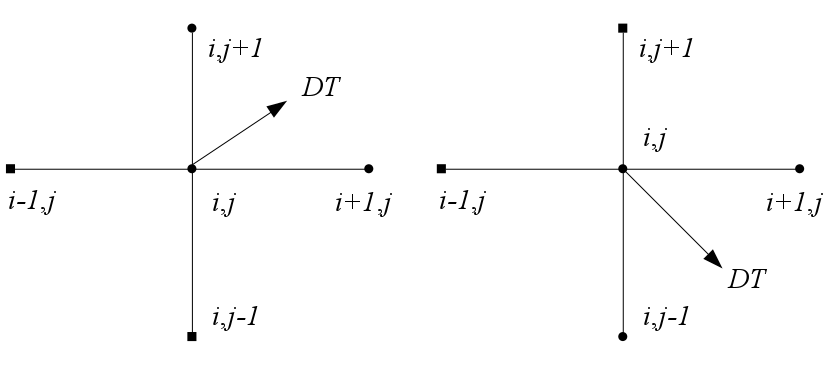
\includegraphics[width=\linewidth]{img/upwind-schema.png}
  \hfil \caption{Пример разных направлений распространения}
  \label{fig:upwind-schema}

\end{figure}

Крэндалл и Лайонс в \cite{V1983} доказали, что последовательные
монотонные схемы сходятся к корректному вязкостному решению. Поэтому
мы можем развивать идеи дальше и применить сказанное выше к уравнениям
эйконала. Существует несколько различных схем приближения, мы
воспользуемся схемой Годунова \cite{F2002}:

\begin{equation}
  \label{eq:godunov-schema}
  \begin{cases}
    \begin{matrix}
       &\max (D^{-x}_{ij}T, -D^{x}_{ij},0)^2 &+\\
     + &\max (D^{-y}_{ij}T, -D^{y}_{ij},0)^2&
    \end{matrix}
    \end{cases}= \frac{1}{F_{ij}^2}
\end{equation}

% Рассмотрим, как будет работать схема Годунова на простом примере:
% $\Delta x = 1$ и $F(x) = 1, 1 < i < n$ и покажем, что она выделяет
% только вогнутые решения:


% Как мы можем решить уравнение \eqref{eq:godunov-schema}? Предположим,
% что у нас есть сетка. Рассмотрим один ее узел и 4 ближайших ее соседа
% см. рисунок~\ref{fig:rec-grid-node}

% \begin{figure}[ht]
%   \centering
%   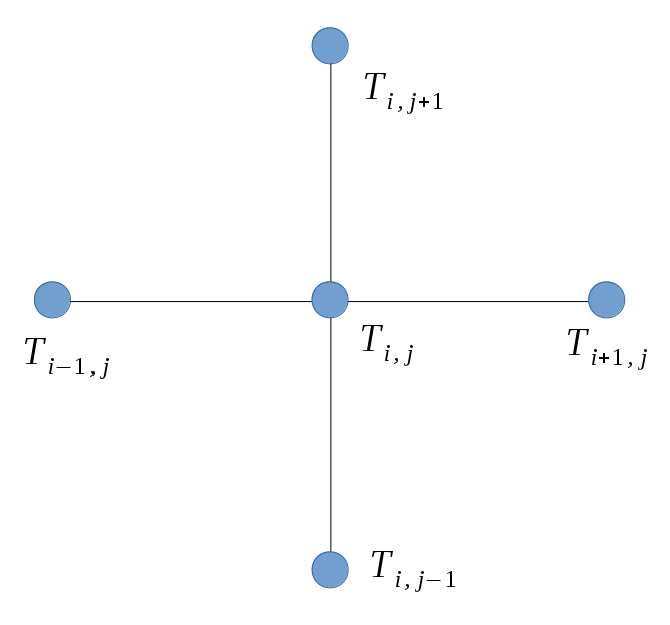
\includegraphics[width=0.5\linewidth]{img/rec-grid-node.png}
%   \hfil \caption{Узлы сетки}
%   \label{fig:rec-grid-node}

% \end{figure}

% Нам нужно выяснить значение $T_{i,j}$. Если исходить из оговоренных в
% постановке задачи условий, хотя бы одна из соседних точек имеет
% числовое значение,

Далее мы подставляем наши разностные производные
\eqref{eq:discrete-defines} в схему Годунова \eqref{eq:godunov-schema}
и получим

\begin{equation}
  \begin{aligned}
  \label{eq:replaced}
    T &= T_{i,j}\\
    T_{x}&= \min(T_{i-1,j},T_{i+1,j})\\
    T_{y}&= \min(T_{i,j-1},T_{i,j-1})
      \end{aligned}
\end{equation}

Уравнение эйконала может быть переписано для дискретного двумерного
случая на прямоугольной сетке как
\begin{equation*}
  \sqrt{\max \left( \frac {T-T_{x}}{\Delta_x},0 \right)^2+  \max \left( \frac
  {T-T_{y}}{\Delta_y},0\right)^2} = \frac{1}{F_{i,j}}
\end{equation*}
Или эквивалентно, можем записать:
\begin{equation}
  \label{eq:discrete-eikonal}
  \max \left( \frac {T-T_{x}}{\Delta_x},0 \right)^2+  \max \left( \frac
      {T-T_{y}}{\Delta_y},0\right)^2 = \frac{1}{F_{i,j}^2}
\end{equation}

Поскольку предполагается, что скорость распространения фронта
положительная $(F>0)$, $T$ будет больше чем $T_x$ и $T_y$ когда фронт
еще не посещал точку $(i,j)$. Следовательно уравнение
\eqref{eq:discrete-eikonal} можно безболезненно переписать еще раз:

\begin{equation}
  \label{eq:discrete-eikonal-2}
  \left( \frac {T-T_{x}}{\Delta_x} \right)^2+
  \left( \frac {T-T_{y}}{\Delta_y} \right)^2 = \frac{1}{F_{i,j}^2}
\end{equation}

Уравнение \eqref{eq:discrete-eikonal-2} обычное квадратное уравнение
вида $aT^2+bT+c=0$ где:

\begin{equation}
  \begin{aligned}
  \label{eq:replaced}
    a &= \Delta_2 x + \Delta^2 y\\[0.4cm]
    b &= -2(\Delta^2y T_{x}+\Delta^2x T_{y})\\
    c &= \Delta^2 y T_{y}^2 + \Delta^2 x T_{x}^2 - \frac{\Delta^2 x
      \Delta^2 y}{F_{ij}^2}
    \end{aligned}
\end{equation}


\subsection{Fast marching method на прямоугольной сетке}
\label{sec:fast-marching-method}

Fast marching method (FMM) \cite{S1999} является наиболее
распространенным способом решать уравнения эйконала. По своей
структуре он сильно похож на алгоритм Дейкстры. Главное отличие от
этого алгоритма в том алгоритм Дейкстры работает на
графе. Следовательно значение каждого узла $x_i$ зависит только от
родительского узла ${x_j}$, следуя принципу оптимальности Белмана.
\begin{equation*}
  T_i = \min_{x_i\in \mathcal{N}} (c_{ij} + T_j)
\end{equation*}

Другими словами узел $x_i$ присоединенный к $x_j$ в его
окрестности $\mathcal{N}(x_i)$ минимизирует (или
максимизирует) значение функции (в этом случае $T_i$)состоящей в
значении функции $T_j$ плюс добавленная стоимость движения из $x_j$ в
$x_i$, представленной как $c_{ij}$.
FMM также следует принципу оптимальности Белмана, но значения для
каждого узла получается из дискретизации уравнения Эйконала,
описанного выше. Эта дискретизация учитывает при подсчитывании
значения всех соседей, поэтому в непрерывном случае FMM вычисляет
время прибытия более аккуратно.

Алгоритм помечает ячейки тремя различными метками:
\begin{enumerate}
\item Изведанная ($\proc{Known}$) : значение в этой ячейке не подлежит более
  пересмотру,
\item Неизведанная ($\proc{Unknown}$): ячейка, значение в которой еще не
  получено,
\item Пробная ($\proc{Trial}$): лежит на границе между Изведанными
  и Неизведанными ячейками, значения функции в этих ячейках
  уже известны, но не определены.
\end{enumerate}

Процедура описанная ниже инициализирует все точки в сетке в состояние
Неизведанное c бесконечным временем достижения. Стартовые
точки устанавливаются в $0$ и считаются Изведанными. Далее основной
цикл FMM начинает выбирать узлы с наименьшим временем прибытия из
Пробных узлов. Для всех соседей этого узла, не являющихся
Изведанными решается уравнение эйконала и получается новое
значение времени прибытия. Если оно оказалось меньше чем текущее
значение, то оно заменяет старое. Если соседняя точка была
Неизведанной, то она становится пробной. Наконец, выбранная
точка становится Изведанной и начинается новая итерация
алгоритма, пока у нас существуют Пробные точки. Полученная
сетка, где в каждой точке наименьшее возможное время прибытия в нее
является результатом работы алгоритма.

FMM нуждается в представлении множества Пробных узлов, для
выполнения над ними следующих операций:
\begin{itemize}
\item Вставка : вставить новый элемент в множество
\item Изменение: изменить порядок элемента, значение которого было
  улучшено
\item Вершина: вернуть элемент с наименьшим значениями
\item Удаление: удалить элемент с наименьшим значением 
\end{itemize}
В реализации нашего алгоритма это наиболее критичный аспект, для
увеличения скорости его работы. Наиболее эффективный способ
использовать неубывающую пирамиду \cite{TK2017}.В русскоязычной
литературе существует два термина, которые сводятся к одному в
английском языке --- это пирамида и куча в перевода \cite{TK2017} есть
комментарии по этому поводу. Вслед за переводчиками, я буду
использовать понятие пирамида. Пирамидой называют упорядоченное дерево,
в котором каждый родитель упорядочивается относительно своих потомков. В
неубывающей пирамиде элемент с минимальным значением находиться в
корне дерева, а все потомки имеют большее числовое значение. Это
выполняется для каждого элемента пирамиды.

Обычно пирамиду реализуют через бинарную пирамиду, Тем не менее,
Фибоначчиева пирамида \cite{F1987} имеет лучшее время действия для
изменения и добавления элементов, но она имеет дополнительные
вычислительные расходы по отношению к другим реализациям пирамид. Для
относительно маленьких сеток, где Пробных элементов не так много
бинарная куча работает лучше. Таблица~\ref{tab:perf} отражает
сложность по времени для этих структур (очередь c приоритетом будет
рассмотрена далее). Стоит отметить, что $n$ здесь --- это количество
узлов на сетке, которые нам предстоит посчитать. В худшем случае у нас
все узлы окажутся в пирамиде.

\begin{table}
  \centering
  \caption{Сводная информация об усредненных вычислительных
    сложностях по времени для пирамид (n -- количество элементов в
    пирамиде)}
  \label{tab:perf}
  \begin{tabular}{|*{5}{c|}}
    \hline
Реализация & Вставка & Изменение & Вершина & Удаление\\[0.3cm]\hline
Фиббоначиева куча & $\Theta(1)$ & $\Theta(1)$&$\Theta(1)$&$\Theta(\log n$) \\\hline
Двоичная куча & $\Theta(\log n)$ & $\Theta(\log n)$&$\Theta(1)$&$\Theta(\log n$) \\\hline
Очередь приоритетов & $\Theta(\log n)$ & -- &$\Theta(1)$&$\Theta(\log n$) \\\hline
    
  \end{tabular}
\end{table}

В каждой итерации вершина пирамиды Пробных точек достигается за
константу $\Theta(1)$, Эйконал решается для не более чем для $2^N$
соседей ($\Theta(1)$ для данного $N$), эти точки вставляются или
изменяются (в худшем случае за $\Theta(\log n)$) И наконец, вершина
удаляется за $\Theta(\log n)$. Следовательно каждая итерация цикла
работает не хуже чем за $\Theta(\log n)$. Поскольку цикл выполнится не
более чем $n$ раз, мы сложность FMM -- $\Theta(\log n)$

Существует некоторое упрощение алгоритма FMM в котором мы не изменяем
значения пробных ячеек, а храним их все. В том числе и разных
типов. Сделать такое нам позволяет очередь приоритетов. Каждый раз,
когда мы получаем новое значение, мы вставляем его в нашу очередь.

Этот метод позволяет нам заменить операцию изменения на операцию
вставки, кроме того, как было указано выше - алгоритм имеет такую же
временную сложность как и другие: $\Theta(\log n)$

\subsection{Fast sweeping method на прямоугольной сетке}
\label{sec:fast-sweeping-method}

Fast sweeping method далее FSM -- итеративный метод, основная идея
которого -- это последовательно ``замести'' сетку в определенных
направлениях. FSM -- выполняет итерации Гаусса-Зейделя в чередующихся
направлениях. Эти направления выбираются так, чтобы все возможные
характеристические кривые решения эйконала делились на возможные квадранты.

Двумерная сетка имеет 4 возможных направления для итерации
Гаусса-Зейделя: различные попарные комбинации вдоль $x$ и $y$ вперед и
назад смотри рисунок~\ref{fig:fsm-sweeps}


\begin{figure}[H]
  \centering
  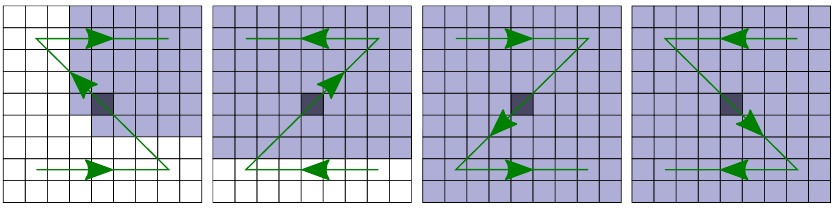
\includegraphics[width=\linewidth]{img/fsm-sweeps.png}
  \hfil \caption{Направления выметаний на двумерной сетке, указаны
    стрелками. Самая темная стрелка -- это стартовая точка,
    затемненные -- проанализированные текущим выметанием}
  \label{fig:fsm-sweeps}

\end{figure}

FSM --- простой алгоритм, выполняющий выметания до тех пор пока
значение не будет утверждено. В каждом выметании эйконал решается для
каждой ячейки и если значение оказалось меньше текущего, то старое
заменяется на новое. Для порядка выметаний используется массив
$\proc{SweepDirs}$, содержащий в себе значения $1$ или $-1$,
подразумевающие направления вперед и назад, по текущему направлению,
мы инициализируем массив единицами, а сетку -- аналогично тому, как
это сделано в алгоритме FMM. Каждую итерацию мы обновляем значения
одного из элементов $\proc{SweepDirs}$, так чтобы пробегались все
возможные значения, для прохождения нужных выметаний. Наконец сам
алгоритм FSM выполняет итерацию Гаусса-Зейделя следуя направлениям
заданным $\proc{SweepDirs}$.

Этот метод проходит сетку до тех пор, пока для каждого $T_i$ не
утвердится его значение, что означает, что на текущем проходе все $T_i$ не
изменились. Для ка каждой ячейки стоимость вычисления уравнения
Эйконала -- $\Theta(1)$. Поскольку существует $n$ узлов, общая
сложность FSM $\Theta(n)$ однако, стоит отметить, что константы этого
выражения высоко зависят от функции скорости $F(x)$. В случае пустого
поля с постоянным $F(x)$, нужно только $4$ выметания, так как
характеристиками в таком случае являются прямые линии однако для более
сложных сеток с препятствиями (или более сложных функций скорости),
где характеристики часто меняют свое направление, нам может
понадобится гораздо большее число выметаний, и поэтому FSM - будет
работать дольше

\subsection{Fast sweeping method на нерегулярной сетке}
\label{sec:unstructured-mesh}

Теперь мы хотим попробовать изменить нашу квадратную сетку на
нерегулярную, для большей свободы определения значений. Для этого
возьмем за основу не прямоугольник, как это было раньше, а треугольник
--- фигура, которой гораздо проще приближаются различные
многоугольники. В частности регулярная прямоугольная сетка (тоже легко
моделируется треугольной сеткой)

Сложность работы с треугольной сеткой в том, что мы не можем просто
разбить на несколько случаев варианты расположений соседних точек,
теперь соседних точек может оказаться как больше так и меньше $4$, и
их положение не определено регулярной структурой. Поэтому, нам нужно
по другому считать локальное решение уравнения эйконала.

Мы все также исследуем уравнение \eqref{eq:eikonal}, только теперь мы
предположим, что $\Omega$ разбита на непересекающиеся, непустые
треугольники $\mathcal{T}$ с диаметром $h_{\mathcal{T}}$, так чтобы
$\Omega = \bigcup_{\mathcal{T}\in \mathcal{T}_h}\mathcal{T}$ Мы
полагаем, что $\mathcal{T}_h$ удовлетворяет следующим условиям.
\begin{itemize}
\item Не более чем $\mu$ треугольников имеют общую вершину;
\item $h = \sup_{\mathcal{T} \in \mathcal{T}_h}\mathcal{T}$<1;
\item Существует такая константа $\omega_0$, независящая от $h$ такая,
  что если $\rho_{\mathcal{T}}$ диаметр наибольшего шара $B \subset
  \mathcal{T}$, тогда для всех $\mathcal{T} \in \mathcal{T}_h,\
  h_{\mathcal{T}} \le \omega_0 \rho_{\mathcal{T}}$
\end{itemize}

Для данного треугольника $\vartriangle ABC$ мы обозначим $\angle A =
\beta $, $\angle B = \alpha$, и $\angle C~=~\gamma;\ \overline{AB} =
c,\ \overline{AC} =b,\ \overline{BC} =a$ длины соответствующих сторон
$AB$, $AC$, и $BC$ соответственно.

Мы считаем, что треугольной сеткой мы задаем кусочно-линейную
аппроксимацию. Фронт распространения кривой обновляет значение времени
прибытия в узле $C$, исходя из значений $T_A$ и $T_B$, для точек $A$ и
$B$ соответственно. Мы полагаем, что луч исходящий из точки $C$ и
ортогональный фронту должен проходить внутри $\vartriangle ABC$

Отметим, что направление изотропного распространение волны совпадает с
направлением градиента поля решения.

Сначала предположим, что $\vartriangle ABC$ остроугоьный. Чтобы
построить схему первого порядка, мы определяем плоский волновой фронт
по известным значениям $T_A$ и $T_B$. Предположим, что угол $\theta$
между фронтом распространения и и ребром $AB$.

Без потери общности мы также предполагаем, что $T_B \ge T_A$. Если
$T_C$ определяется через $T_A$ и $T_B$, тогда по принципу Гюгенса
фронт волны должен пройти сначала через вершину $A$, затем через
вершину $B$, и наконец $C$. Чтобы это гарантировать, надо чтобы
выполнялись следующие условия:
\begin{itemize}
\item $|T_B-T_A| / f_C \le \overline{AB} = c$ т.е., это означает
  возможность фронта от $A$ до $B$ с данной скоростью, где $f_c$ - это
  обратное значение скорости в точке $F(C)$;
  \item $\theta \le \alpha$ это означает, что фронт пройдет через $B$
    раньше чем через $A$
  \item $\theta + \beta < \frac{\pi}{2}$ В противном случае нарушется
    условие причинности, потому, что ортогональная линия от $C$ к
    фронту проходит вне треугольника; смотри рисунок~\ref{fig:triangle-front}
\end{itemize}

\begin{figure}[H]
  \centering
  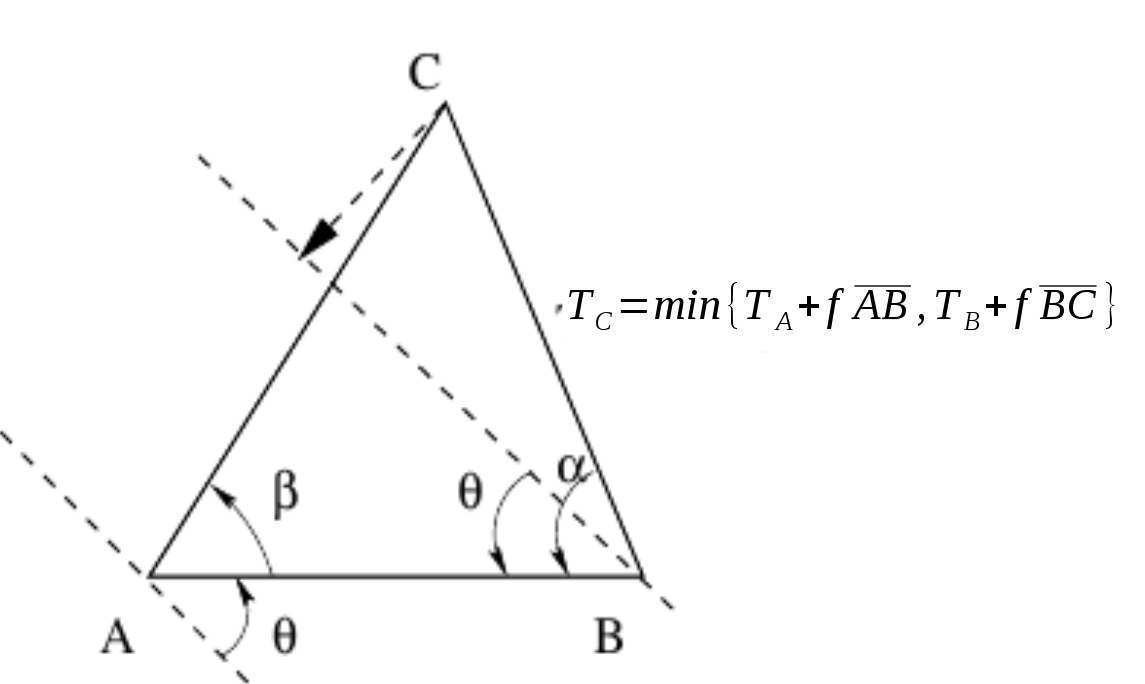
\includegraphics[width=0.7\linewidth]{img/triangle-front.png}
  \hfil \caption{Изменение значения в вершине С, c нарушенным условием
  причинности}
  \label{fig:triangle-front}

\end{figure}

Если все $n$ треугольников
$\mathcal{T}_1,\mathcal{T}_2,...,\mathcal{T}_n$ вокруг $C$
остроугольные, фронт волны может быть захвачен одним из
треугольников.

Из всего выше сказанного мы можем получить следующий алгоритм для
нахождения локального решения. Общая его идея в том, что если 
нарушаются условия для того, чтобы считать распространение фронта
через точки $A$ и $B$, тогда предполагаем, что фронт идет от одной из
вершин, и выбираем из какой пришел быстрее.

\begin{enumerate}
\item если $|T_B-T_A| \le c f_C$, тогда
  \begin{equation*}
    \theta = arcsin \left(\frac{|T_B-T_A|}{c f_C}\right);
  \end{equation*}
  \begin{enumerate}
  \item если $\max (0,\alpha - \frac{\pi}{2}) \le \theta \le
    \frac{\pi}{2} - \beta$ или $\alpha - \frac{\pi}{2} \le \theta \le
    \min(0, \frac{\pi}{2} - \beta)$, тогда
    \begin{equation*}
      \begin{aligned}{c}
        h = \overline{CP} = a \sin(\alpha - \theta); H = \overline{CQ}=
        b \sin (\beta + \theta);\\
        T_C = \min\{T_C,0.5(h f_C + T_B)+0.5(H f_C + T_A)\};
      \end{aligned}
    \end{equation*}
  \item иначе
    \begin{equation*}
      T_C = \min\{T_C,T_A+b f_C, T_B + a f_C\};
    \end{equation*}
  \end{enumerate}
\item иначе
  \begin{equation*}
    T_C = \min{T_C,T_A+b f_C, T_B + a f_C};
  \end{equation*}

\end{enumerate}

Теперь для того, чтобы определить значение $T_C$ мы применим эту
процедуру для каждого пары точек соседних с $T_C$ и установим
наименьшее из полученных значений как решение в этой точке

Связываясь с треугольной сеткой мы получаем еще одну задачу - как в
рамках алгоритма FSM нам проводить процедуру выметания? Теперь у нас
нет жесткого порядка, по которому мы можем пройтись, однако мы его
можем установить. Для этого нам необходимо выделить несколько точек на
плоскости и относительно каждой  отсортировать остальные точки в порядке
удаления от нее и проводить выметания по таким направлениям в сторону
возрастания и в сторону убывания. В работе \cite{FS2007} также
утверждается, что для двумерного случая достаточно всего 3-х
точек. Таким образом будет 6 направлений выметаний.

Условия остановки алгоритма остались те же самые, что и в обыкновенном
FSM, в этом алгоритме добавляется другой критичный параметр для
вычислительной трудности: сортировка всех точек. Здесь уже давно
получены результаты вплоть до сортировки за линейное время набора
целочисленных точек \cite{K2017}. Проблема же с количеством выметаний
ровно та же, что и в классическом FSM

% рисунок с несколькими опорными точками и фронтом пробегания по
% остальным точкам


\subsubsection{Триангуляция}
\label{sec:triangulate}

\subsection{Вопросы реализации}
\label{sec:programming}



%%% Local Variables:
%%% mode: latex
%%% TeX-master: "eikonal_solver"
%%% End:
